% Created by tikzDevice version 0.12.6 on 2026-07-04 06:01:33
% !TEX encoding = UTF-8 Unicode
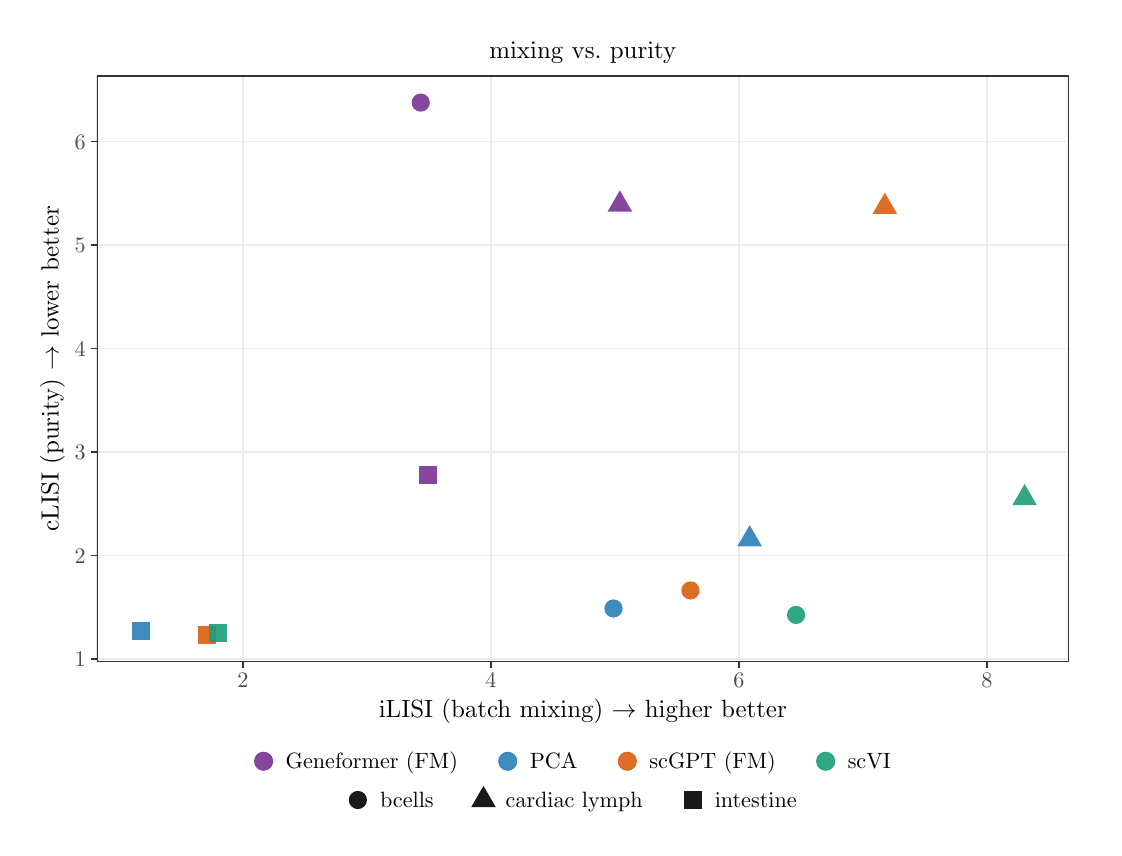
\begin{tikzpicture}[x=1pt,y=1pt]
\definecolor{fillColor}{RGB}{255,255,255}
\path[use as bounding box,fill=fillColor,fill opacity=0.00] (0,0) rectangle (385.20,289.08);
\begin{scope}
\path[clip] (  0.00,  0.00) rectangle (385.20,289.08);
\definecolor{drawColor}{RGB}{255,255,255}
\definecolor{fillColor}{RGB}{255,255,255}

\path[draw=drawColor,line width= 0.5pt,line join=round,line cap=round,fill=fillColor] ( -0.00, -0.00) rectangle (385.20,289.08);
\end{scope}
\begin{scope}
\path[clip] ( 25.00, 60.07) rectangle (376.20,271.63);
\definecolor{fillColor}{RGB}{255,255,255}

\path[fill=fillColor] ( 25.00, 60.07) rectangle (376.20,271.63);
\definecolor{drawColor}{gray}{0.92}

\path[draw=drawColor,line width= 0.5pt,line join=round] ( 25.00, 60.99) --
	(376.20, 60.99);

\path[draw=drawColor,line width= 0.5pt,line join=round] ( 25.00, 98.37) --
	(376.20, 98.37);

\path[draw=drawColor,line width= 0.5pt,line join=round] ( 25.00,135.74) --
	(376.20,135.74);

\path[draw=drawColor,line width= 0.5pt,line join=round] ( 25.00,173.12) --
	(376.20,173.12);

\path[draw=drawColor,line width= 0.5pt,line join=round] ( 25.00,210.49) --
	(376.20,210.49);

\path[draw=drawColor,line width= 0.5pt,line join=round] ( 25.00,247.87) --
	(376.20,247.87);

\path[draw=drawColor,line width= 0.5pt,line join=round] ( 77.80, 60.07) --
	( 77.80,271.63);

\path[draw=drawColor,line width= 0.5pt,line join=round] (167.39, 60.07) --
	(167.39,271.63);

\path[draw=drawColor,line width= 0.5pt,line join=round] (256.99, 60.07) --
	(256.99,271.63);

\path[draw=drawColor,line width= 0.5pt,line join=round] (346.58, 60.07) --
	(346.58,271.63);
\definecolor{fillColor}{RGB}{217,95,14}

\path[fill=fillColor,fill opacity=0.90] (239.49, 85.72) circle (  3.29);
\definecolor{fillColor}{RGB}{123,50,148}

\path[fill=fillColor,fill opacity=0.90] (142.03,262.01) circle (  3.29);
\definecolor{fillColor}{RGB}{44,127,184}

\path[fill=fillColor,fill opacity=0.90] (211.68, 79.20) circle (  3.29);
\definecolor{fillColor}{RGB}{217,95,14}

\path[fill=fillColor,fill opacity=0.90] (309.72,229.47) --
	(314.15,221.80) --
	(305.29,221.80) --
	cycle;
\definecolor{fillColor}{RGB}{123,50,148}

\path[fill=fillColor,fill opacity=0.90] (213.99,230.29) --
	(218.42,222.61) --
	(209.56,222.61) --
	cycle;
\definecolor{fillColor}{RGB}{44,127,184}

\path[fill=fillColor,fill opacity=0.90] (260.88,109.34) --
	(265.31,101.67) --
	(256.45,101.67) --
	cycle;
\definecolor{fillColor}{RGB}{217,95,14}

\path[fill=fillColor,fill opacity=0.90] ( 61.64, 66.39) --
	( 68.22, 66.39) --
	( 68.22, 72.97) --
	( 61.64, 72.97) --
	cycle;
\definecolor{fillColor}{RGB}{123,50,148}

\path[fill=fillColor,fill opacity=0.90] (141.50,124.16) --
	(148.08,124.16) --
	(148.08,130.74) --
	(141.50,130.74) --
	cycle;
\definecolor{fillColor}{RGB}{44,127,184}

\path[fill=fillColor,fill opacity=0.90] ( 37.67, 67.88) --
	( 44.25, 67.88) --
	( 44.25, 74.46) --
	( 37.67, 74.46) --
	cycle;
\definecolor{fillColor}{RGB}{27,158,119}

\path[fill=fillColor,fill opacity=0.90] (277.66, 76.87) circle (  3.29);

\path[fill=fillColor,fill opacity=0.90] (360.24,124.19) --
	(364.67,116.51) --
	(355.80,116.51) --
	cycle;

\path[fill=fillColor,fill opacity=0.90] ( 65.37, 67.03) --
	( 71.95, 67.03) --
	( 71.95, 73.61) --
	( 65.37, 73.61) --
	cycle;
\definecolor{drawColor}{gray}{0.20}

\path[draw=drawColor,line width= 0.5pt,line join=round,line cap=round] ( 25.00, 60.07) rectangle (376.20,271.63);
\end{scope}
\begin{scope}
\path[clip] (  0.00,  0.00) rectangle (385.20,289.08);
\definecolor{drawColor}{gray}{0.30}

\node[text=drawColor,anchor=base east,inner sep=0pt, outer sep=0pt, scale=  0.80] at ( 20.95, 58.24) {1};

\node[text=drawColor,anchor=base east,inner sep=0pt, outer sep=0pt, scale=  0.80] at ( 20.95, 95.61) {2};

\node[text=drawColor,anchor=base east,inner sep=0pt, outer sep=0pt, scale=  0.80] at ( 20.95,132.99) {3};

\node[text=drawColor,anchor=base east,inner sep=0pt, outer sep=0pt, scale=  0.80] at ( 20.95,170.36) {4};

\node[text=drawColor,anchor=base east,inner sep=0pt, outer sep=0pt, scale=  0.80] at ( 20.95,207.74) {5};

\node[text=drawColor,anchor=base east,inner sep=0pt, outer sep=0pt, scale=  0.80] at ( 20.95,245.11) {6};
\end{scope}
\begin{scope}
\path[clip] (  0.00,  0.00) rectangle (385.20,289.08);
\definecolor{drawColor}{gray}{0.20}

\path[draw=drawColor,line width= 0.5pt,line join=round] ( 22.75, 60.99) --
	( 25.00, 60.99);

\path[draw=drawColor,line width= 0.5pt,line join=round] ( 22.75, 98.37) --
	( 25.00, 98.37);

\path[draw=drawColor,line width= 0.5pt,line join=round] ( 22.75,135.74) --
	( 25.00,135.74);

\path[draw=drawColor,line width= 0.5pt,line join=round] ( 22.75,173.12) --
	( 25.00,173.12);

\path[draw=drawColor,line width= 0.5pt,line join=round] ( 22.75,210.49) --
	( 25.00,210.49);

\path[draw=drawColor,line width= 0.5pt,line join=round] ( 22.75,247.87) --
	( 25.00,247.87);
\end{scope}
\begin{scope}
\path[clip] (  0.00,  0.00) rectangle (385.20,289.08);
\definecolor{drawColor}{gray}{0.20}

\path[draw=drawColor,line width= 0.5pt,line join=round] ( 77.80, 57.82) --
	( 77.80, 60.07);

\path[draw=drawColor,line width= 0.5pt,line join=round] (167.39, 57.82) --
	(167.39, 60.07);

\path[draw=drawColor,line width= 0.5pt,line join=round] (256.99, 57.82) --
	(256.99, 60.07);

\path[draw=drawColor,line width= 0.5pt,line join=round] (346.58, 57.82) --
	(346.58, 60.07);
\end{scope}
\begin{scope}
\path[clip] (  0.00,  0.00) rectangle (385.20,289.08);
\definecolor{drawColor}{gray}{0.30}

\node[text=drawColor,anchor=base,inner sep=0pt, outer sep=0pt, scale=  0.80] at ( 77.80, 50.51) {2};

\node[text=drawColor,anchor=base,inner sep=0pt, outer sep=0pt, scale=  0.80] at (167.39, 50.51) {4};

\node[text=drawColor,anchor=base,inner sep=0pt, outer sep=0pt, scale=  0.80] at (256.99, 50.51) {6};

\node[text=drawColor,anchor=base,inner sep=0pt, outer sep=0pt, scale=  0.80] at (346.58, 50.51) {8};
\end{scope}
\begin{scope}
\path[clip] (  0.00,  0.00) rectangle (385.20,289.08);
\definecolor{drawColor}{RGB}{0,0,0}

\node[text=drawColor,anchor=base,inner sep=0pt, outer sep=0pt, scale=  0.90] at (200.60, 39.75) {iLISI (batch mixing) $\to$ higher better};
\end{scope}
\begin{scope}
\path[clip] (  0.00,  0.00) rectangle (385.20,289.08);
\definecolor{drawColor}{RGB}{0,0,0}

\node[text=drawColor,rotate= 90.00,anchor=base,inner sep=0pt, outer sep=0pt, scale=  0.90] at ( 11.20,165.85) {cLISI (purity) $\to$ lower better};
\end{scope}
\begin{scope}
\path[clip] (  0.00,  0.00) rectangle (385.20,289.08);
\definecolor{fillColor}{RGB}{255,255,255}

\path[fill=fillColor] ( 80.25, 19.00) rectangle (320.94, 29.00);
\end{scope}
\begin{scope}
\path[clip] (  0.00,  0.00) rectangle (385.20,289.08);
\definecolor{fillColor}{RGB}{255,255,255}

\path[fill=fillColor] ( 80.25, 19.00) rectangle ( 90.25, 29.00);
\definecolor{drawColor}{RGB}{123,50,148}
\definecolor{fillColor}{RGB}{123,50,148}

\path[draw=drawColor,draw opacity=0.90,line width= 0.3pt,line join=round,line cap=round,fill=fillColor,fill opacity=0.90] ( 85.25, 24.00) circle (  3.29);
\end{scope}
\begin{scope}
\path[clip] (  0.00,  0.00) rectangle (385.20,289.08);
\definecolor{fillColor}{RGB}{255,255,255}

\path[fill=fillColor] (168.47, 19.00) rectangle (178.47, 29.00);
\definecolor{drawColor}{RGB}{44,127,184}
\definecolor{fillColor}{RGB}{44,127,184}

\path[draw=drawColor,draw opacity=0.90,line width= 0.3pt,line join=round,line cap=round,fill=fillColor,fill opacity=0.90] (173.47, 24.00) circle (  3.29);
\end{scope}
\begin{scope}
\path[clip] (  0.00,  0.00) rectangle (385.20,289.08);
\definecolor{fillColor}{RGB}{255,255,255}

\path[fill=fillColor] (211.69, 19.00) rectangle (221.69, 29.00);
\definecolor{drawColor}{RGB}{217,95,14}
\definecolor{fillColor}{RGB}{217,95,14}

\path[draw=drawColor,draw opacity=0.90,line width= 0.3pt,line join=round,line cap=round,fill=fillColor,fill opacity=0.90] (216.69, 24.00) circle (  3.29);
\end{scope}
\begin{scope}
\path[clip] (  0.00,  0.00) rectangle (385.20,289.08);
\definecolor{fillColor}{RGB}{255,255,255}

\path[fill=fillColor] (283.34, 19.00) rectangle (293.34, 29.00);
\definecolor{drawColor}{RGB}{27,158,119}
\definecolor{fillColor}{RGB}{27,158,119}

\path[draw=drawColor,draw opacity=0.90,line width= 0.3pt,line join=round,line cap=round,fill=fillColor,fill opacity=0.90] (288.34, 24.00) circle (  3.29);
\end{scope}
\begin{scope}
\path[clip] (  0.00,  0.00) rectangle (385.20,289.08);
\definecolor{drawColor}{RGB}{0,0,0}

\node[text=drawColor,anchor=base west,inner sep=0pt, outer sep=0pt, scale=  0.80] at ( 93.25, 21.24) {Geneformer (FM)};
\end{scope}
\begin{scope}
\path[clip] (  0.00,  0.00) rectangle (385.20,289.08);
\definecolor{drawColor}{RGB}{0,0,0}

\node[text=drawColor,anchor=base west,inner sep=0pt, outer sep=0pt, scale=  0.80] at (181.47, 21.24) {PCA};
\end{scope}
\begin{scope}
\path[clip] (  0.00,  0.00) rectangle (385.20,289.08);
\definecolor{drawColor}{RGB}{0,0,0}

\node[text=drawColor,anchor=base west,inner sep=0pt, outer sep=0pt, scale=  0.80] at (224.69, 21.24) {scGPT (FM)};
\end{scope}
\begin{scope}
\path[clip] (  0.00,  0.00) rectangle (385.20,289.08);
\definecolor{drawColor}{RGB}{0,0,0}

\node[text=drawColor,anchor=base west,inner sep=0pt, outer sep=0pt, scale=  0.80] at (296.34, 21.24) {scVI};
\end{scope}
\begin{scope}
\path[clip] (  0.00,  0.00) rectangle (385.20,289.08);
\definecolor{fillColor}{RGB}{255,255,255}

\path[fill=fillColor] (114.32,  5.00) rectangle (286.88, 15.00);
\end{scope}
\begin{scope}
\path[clip] (  0.00,  0.00) rectangle (385.20,289.08);
\definecolor{fillColor}{RGB}{255,255,255}

\path[fill=fillColor] (114.32,  5.00) rectangle (124.32, 15.00);
\definecolor{fillColor}{RGB}{0,0,0}

\path[fill=fillColor,fill opacity=0.90] (119.32, 10.00) circle (  3.29);
\end{scope}
\begin{scope}
\path[clip] (  0.00,  0.00) rectangle (385.20,289.08);
\definecolor{fillColor}{RGB}{255,255,255}

\path[fill=fillColor] (159.70,  5.00) rectangle (169.70, 15.00);
\definecolor{fillColor}{RGB}{0,0,0}

\path[fill=fillColor,fill opacity=0.90] (164.70, 15.12) --
	(169.13,  7.44) --
	(160.27,  7.44) --
	cycle;
\end{scope}
\begin{scope}
\path[clip] (  0.00,  0.00) rectangle (385.20,289.08);
\definecolor{fillColor}{RGB}{255,255,255}

\path[fill=fillColor] (235.28,  5.00) rectangle (245.28, 15.00);
\definecolor{fillColor}{RGB}{0,0,0}

\path[fill=fillColor,fill opacity=0.90] (236.99,  6.71) --
	(243.57,  6.71) --
	(243.57, 13.29) --
	(236.99, 13.29) --
	cycle;
\end{scope}
\begin{scope}
\path[clip] (  0.00,  0.00) rectangle (385.20,289.08);
\definecolor{drawColor}{RGB}{0,0,0}

\node[text=drawColor,anchor=base west,inner sep=0pt, outer sep=0pt, scale=  0.80] at (127.32,  7.24) {bcells};
\end{scope}
\begin{scope}
\path[clip] (  0.00,  0.00) rectangle (385.20,289.08);
\definecolor{drawColor}{RGB}{0,0,0}

\node[text=drawColor,anchor=base west,inner sep=0pt, outer sep=0pt, scale=  0.80] at (172.70,  7.24) {cardiac lymph};
\end{scope}
\begin{scope}
\path[clip] (  0.00,  0.00) rectangle (385.20,289.08);
\definecolor{drawColor}{RGB}{0,0,0}

\node[text=drawColor,anchor=base west,inner sep=0pt, outer sep=0pt, scale=  0.80] at (248.28,  7.24) {intestine};
\end{scope}
\begin{scope}
\path[clip] (  0.00,  0.00) rectangle (385.20,289.08);
\definecolor{drawColor}{RGB}{0,0,0}

\node[text=drawColor,anchor=base,inner sep=0pt, outer sep=0pt, scale=  0.90] at (200.60,277.88) {mixing vs.\ purity};
\end{scope}
\end{tikzpicture}
